\begin{figure}[htbp]
  \centering
    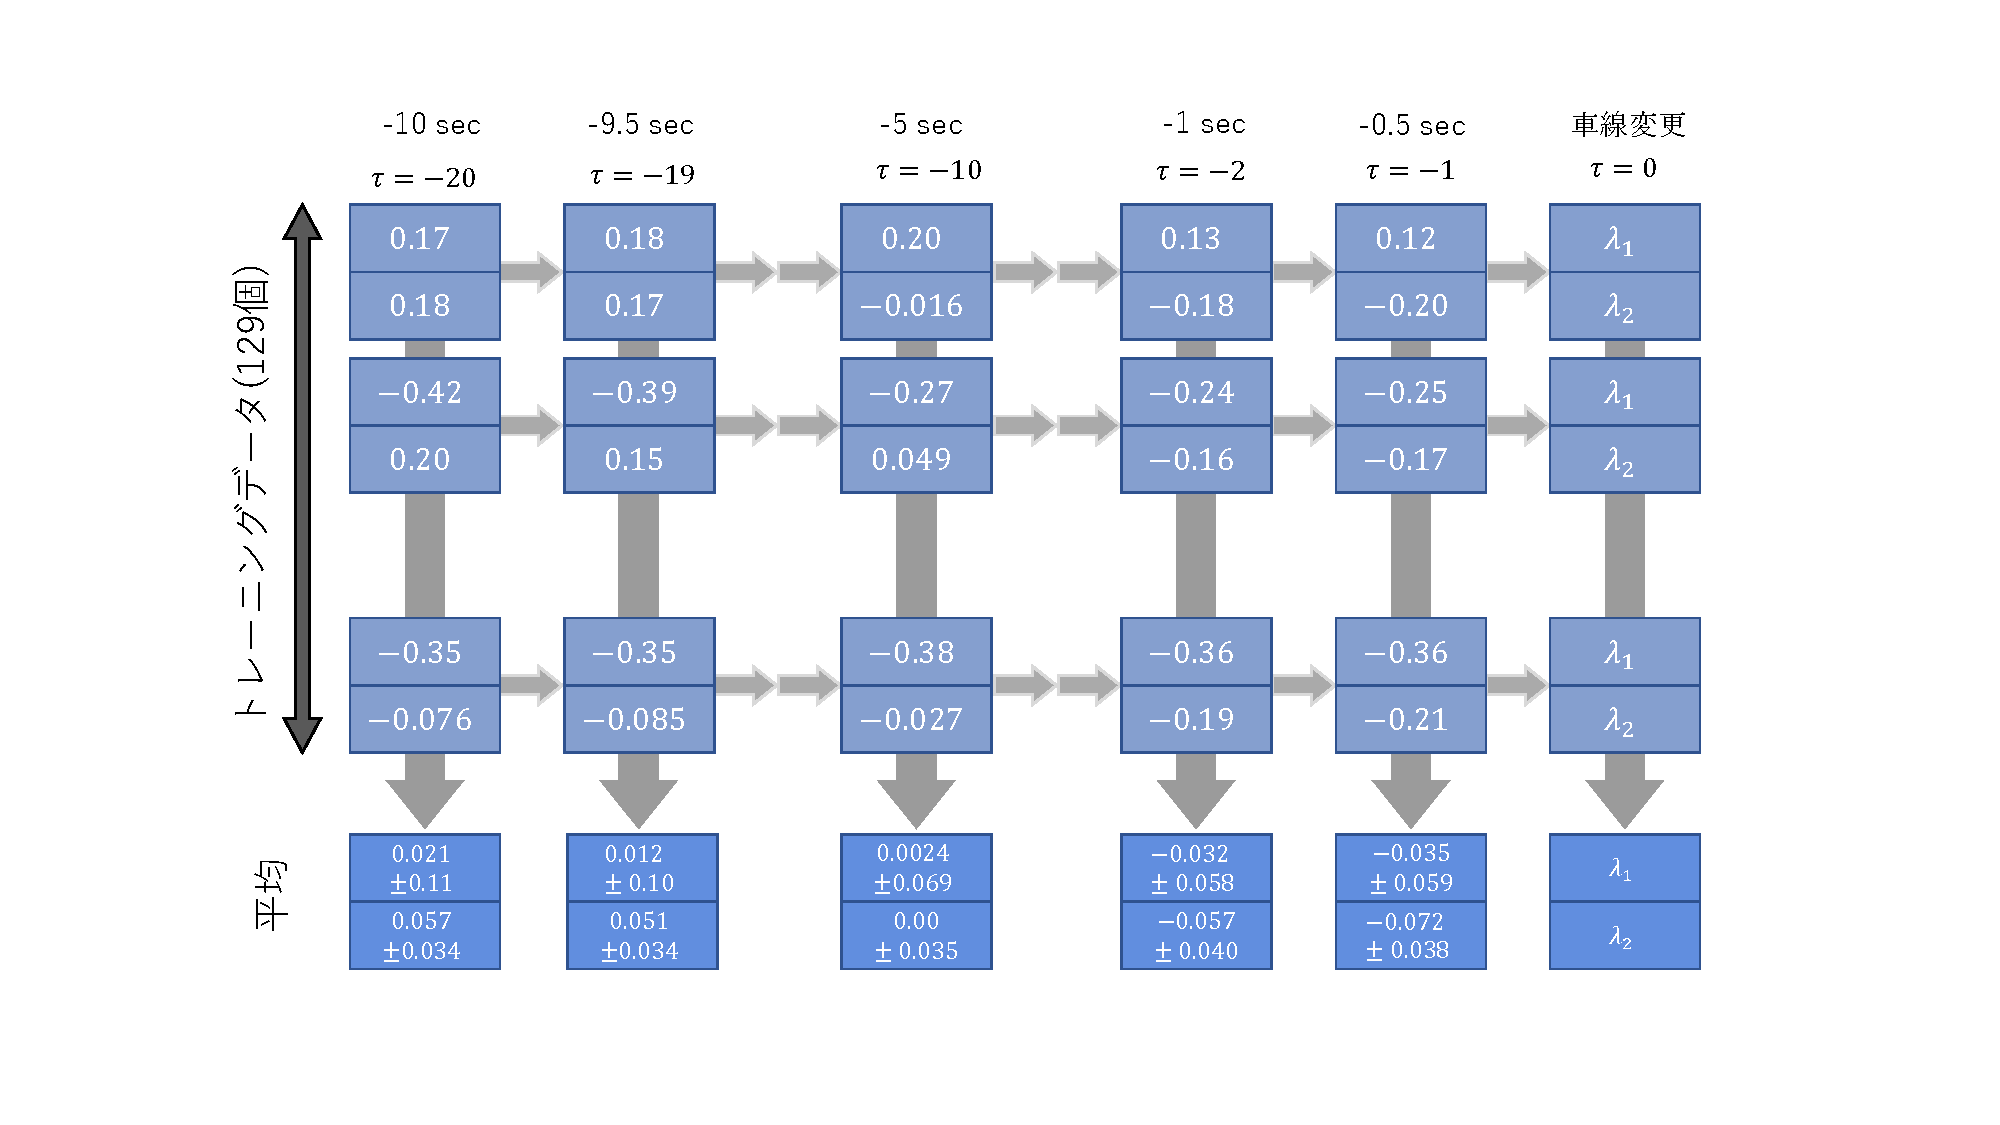
\includegraphics[width=11cm,keepaspectratio]{fig/training_flow.pdf}
  \caption{正規分布を訓練データから得る流れを図示したもの.各セルの中の値は特徴量$\lambda_1$, $\lambda_2$の一例を示している.各行はある車線変更の1試行において得られた特徴の推移を並べており,これらの129回分について平均,分散を求めることで,各時刻の属する正規分布を求めている.}
  \label{fig:training_flow}
\end{figure}
